\begin{figure}[!t]
    \centering
    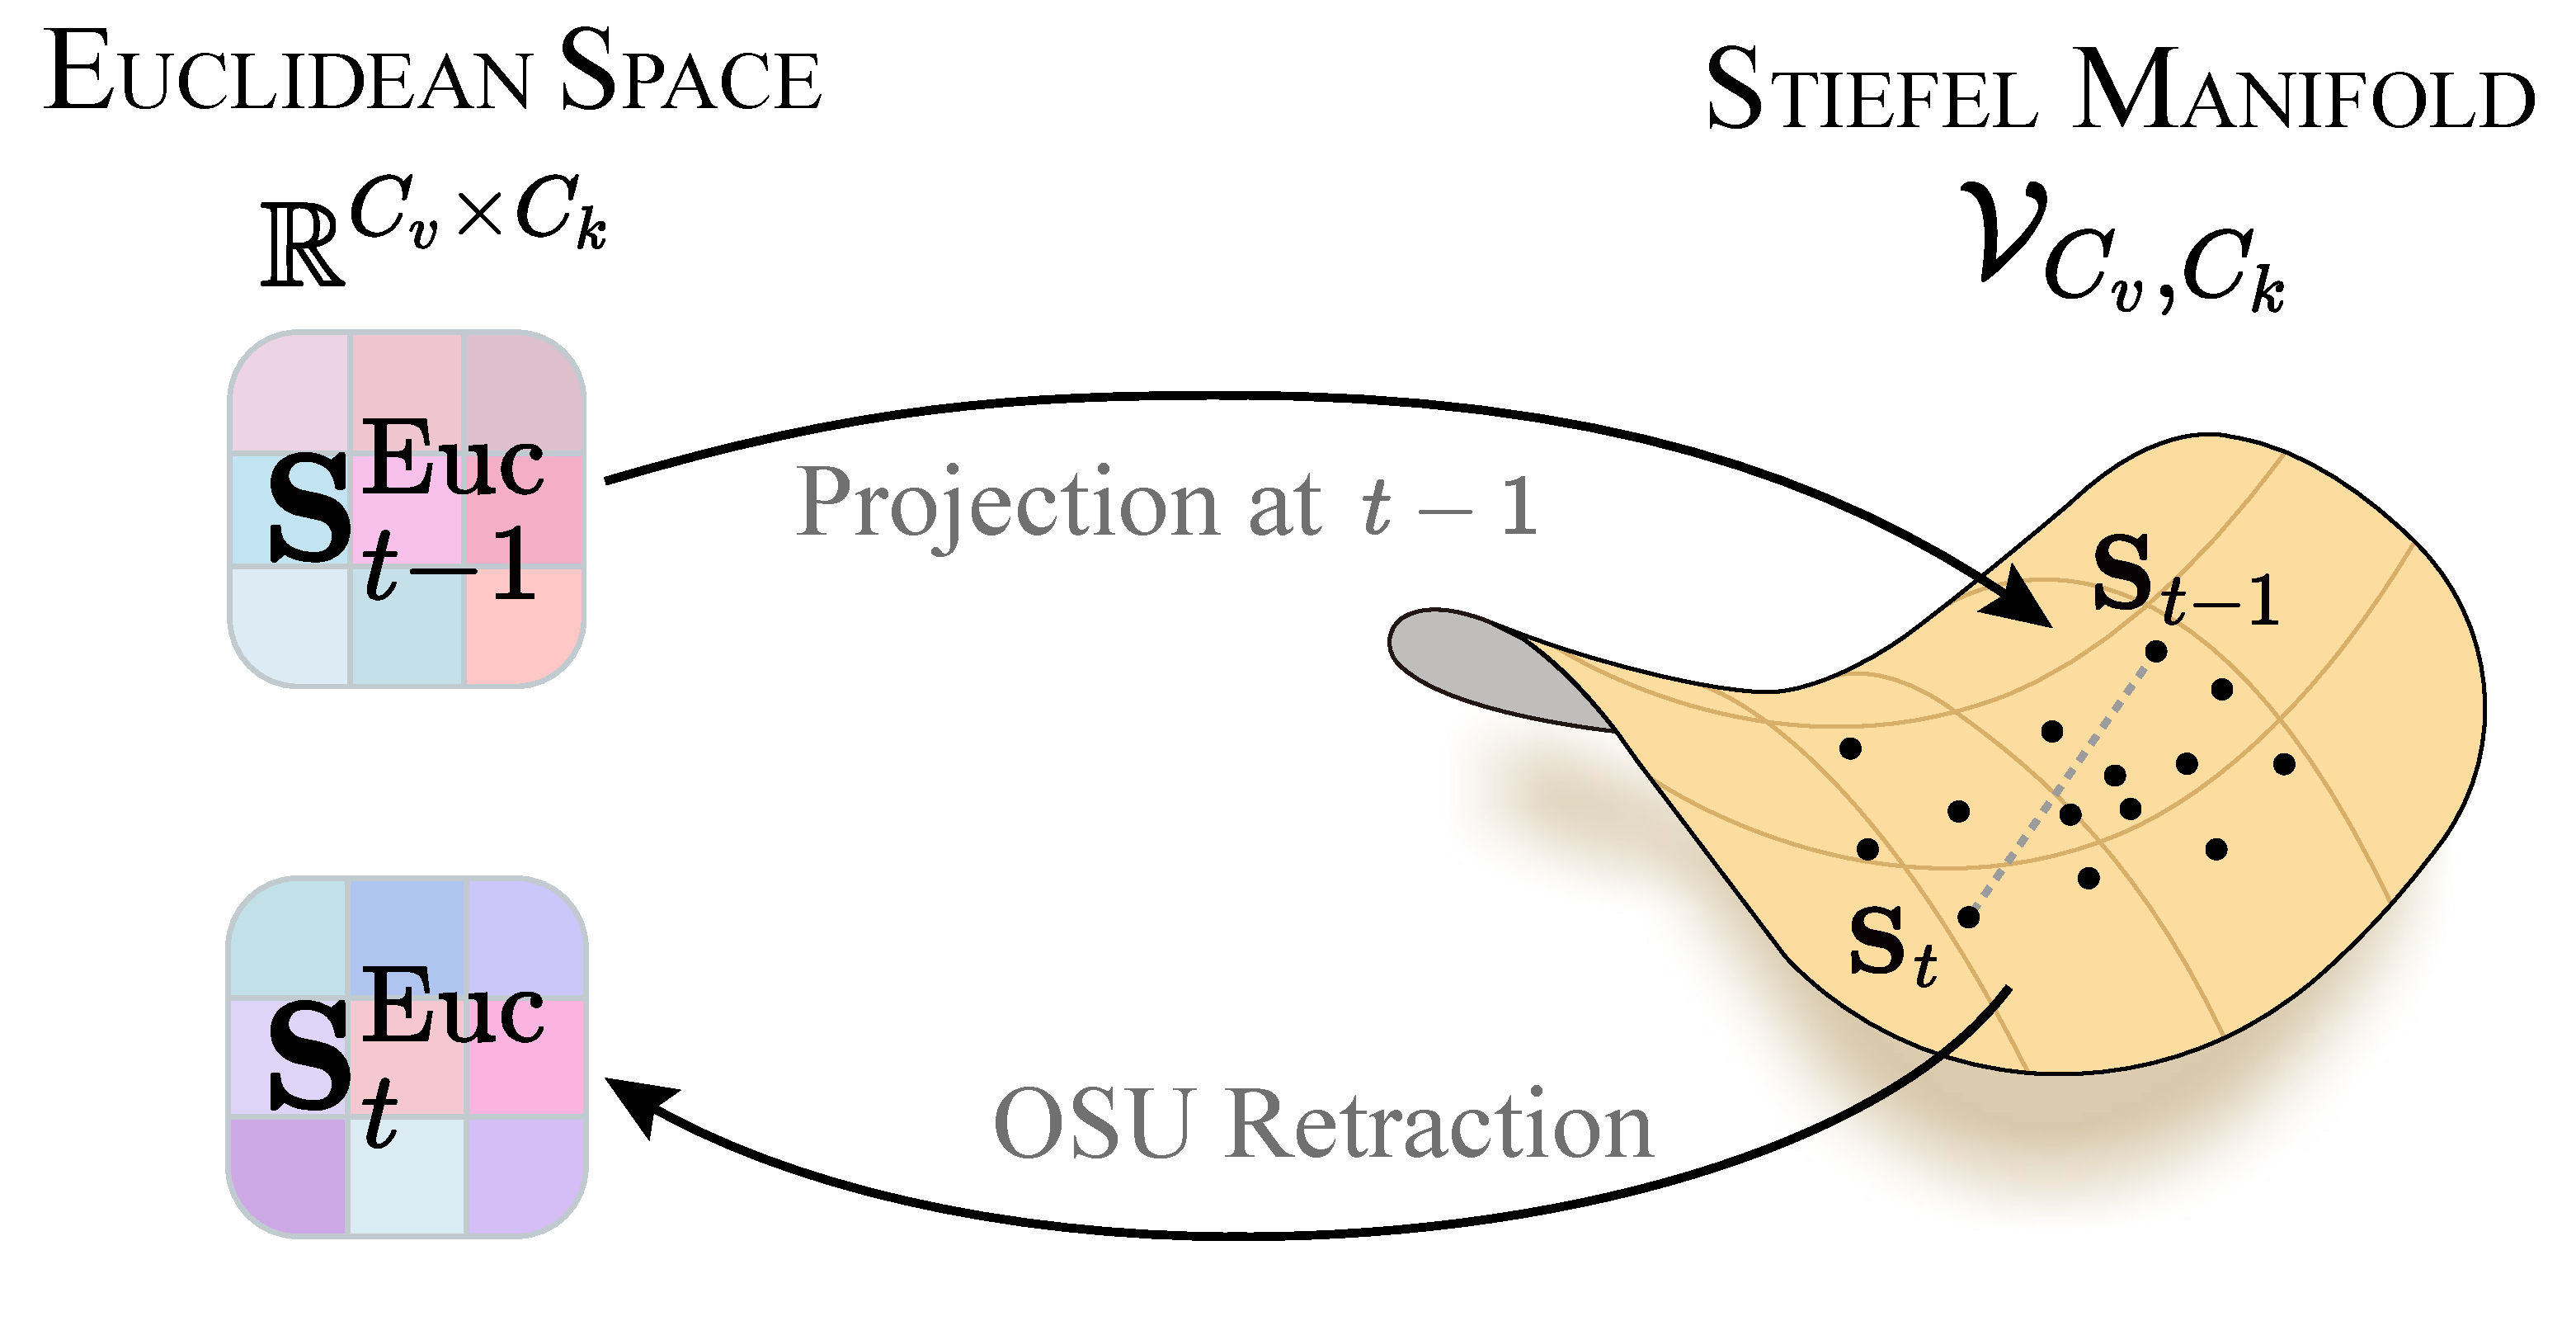
\includegraphics[width=0.94\linewidth]{fig/osu/fig_osu.pdf}
    \caption{Illustration of OSU.
    Standard Euclidean recurrences suffer from rank collapse over long sequences (manifested as singular value decay and increasing condition number). OSU constrains state evolution on the Stiefel manifold via orthogonalized update. The unconstrained intermediate state $\mathbf{S}_t^{\text{Euc}}$ is projected back to the manifold as $\mathbf{S}_t$, ensuring stable temporal transitions.}
    \label{fig:osu}
\end{figure}

\begin{figure}[!t]
    \centering
    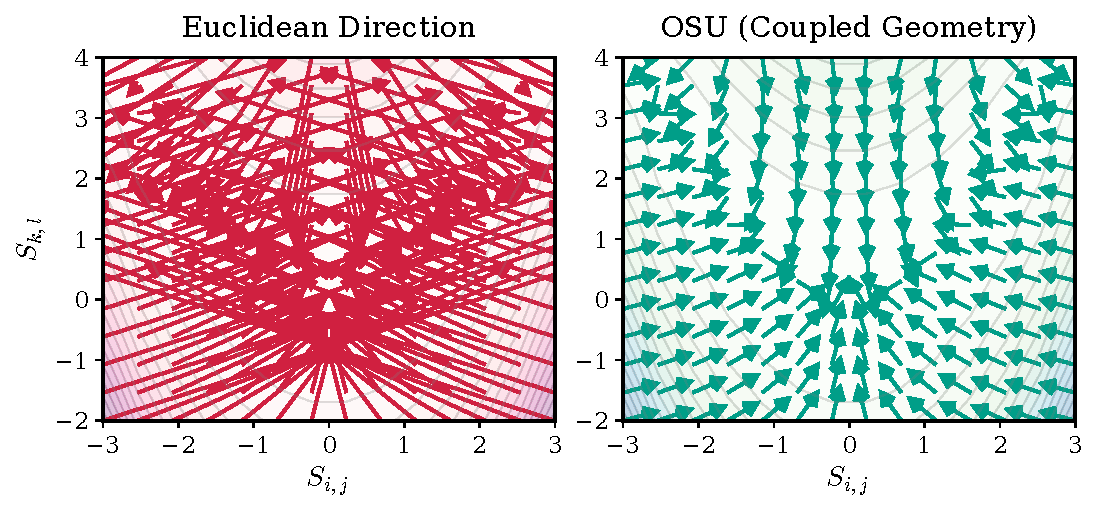
\includegraphics[width=1.0\linewidth]{fig/landscape_2d/fig_landscape_2d.pdf}
    \caption{\textbf{Behavioral comparison of optimization vector fields.}
    Unconstrained Euclidean updates cause the state to drift away from orthogonal constraints (climbing valley walls). OSU generates a corrective flow that pulls iterates back onto the Stiefel manifold (valley floor).}
    \label{fig:landscape_2d_behavior}
\end{figure}